\documentclass[]{book}
\usepackage{amsmath,amssymb}
\usepackage{amsthm}
\usepackage{xpatch}
\xpatchcmd\swappedhead{~}{.~}{}{}

\usepackage[T1]{fontenc}
\usepackage[utf8]{inputenc}

\usepackage{parskip}
\usepackage{lmodern}
\usepackage{verbatim}
\usepackage{enumerate}
\usepackage{longtable}
\usepackage{booktabs}


\usepackage{xcolor}
%sudo apt-get install texlive-pictures
\usepackage[all]{xy}

\usepackage{hyperref}

\usepackage[ marginparwidth=3cm, marginparsep=0cm]{geometry}
\usepackage{graphicx}
\usepackage[spanish]{babel}



\usepackage{fancyhdr}
\makeatletter

\fancyhf{}% Clear header/footer
\fancyhead[RO]{\leftmark}% Chapter details in book
\fancyhead[LE]{\rightmark \;\; Hugo J. Bello}% Stored \chapterauthor details
\fancyfoot[C]{\thepage}
%\renewcommand{\headrulewidth}{0pt}% Remove header rule
%\renewcommand{\footrulewidth}{0pt}% Remove footer rule (default)
\pagestyle{fancy}
\makeatother

% Scale images if necessary, so that they will not overflow the page
% margins by default, and it is still possible to overwrite the defaults
% using explicit options in \includegraphics[width, height, ...]{}
\setkeys{Gin}{width=\maxwidth,height=\maxheight,keepaspectratio}
% Set default figure placement to htbp
\makeatletter
\def\fps@figure{htbp}
\makeatother

% Scale images if necessary, so that they will not overflow the page
% margins by default, and it is still possible to overwrite the defaults
% using explicit options in \includegraphics[width, height, ...]{}
\setkeys{Gin}{width=\maxwidth,height=\maxheight,keepaspectratio}
% Set default figure placement to htbp
\makeatletter
\def\fps@figure{htbp}
\makeatother


\providecommand{\tightlist}{%
  \setlength{\itemsep}{0pt}\setlength{\parskip}{0pt}}

  
%remove section numbers
%\setcounter{secnumdepth}{0}

\title{Variables aleatorias continuas}
\author{Hugo J. Bello}
\date{}


\renewcommand{\familydefault}{\sfdefault}
\setcounter{chapter}{4}


\theoremstyle{plain}
\swapnumbers % Switch number/label style
\newtheorem{theorem}{Theorem}[section]
\newtheorem{corollary}[theorem]{Corollary}
\newtheorem{lemma}[theorem]{Lemma}
\newtheorem{claim}{Claim}[theorem]
\newtheorem{axiom}[theorem]{Axiom}
\newtheorem{conjecture}[theorem]{Conjecture}
\newtheorem{fact}[theorem]{Fact}
\newtheorem{hypothesis}[theorem]{Hypothesis}
\newtheorem{assumption}[theorem]{Assumption}
\newtheorem{proposition}[theorem]{Proposition}
\newtheorem{property}[theorem]{Propiedad}
\newtheorem{properties}[theorem]{Propiedades}
\newtheorem{criterion}[theorem]{Criterion}
\theoremstyle{definition}
\newtheorem{definition}[theorem]{Definición}
\newtheorem{note}[theorem]{Nota}
\newtheorem{definitions}[theorem]{Definiciones}
\newtheorem{example}[theorem]{Ejemplo}
\newtheorem{remark}[theorem]{Remark}
\newtheorem{problem}[theorem]{Problem}
\newtheorem{principle}[theorem]{Principle}
\newtheorem{method}[theorem]{Método}
\newtheorem{exercise}[theorem]{Ejercicio}

% for specifying a name
\theoremstyle{definition} % just in case the style had changed
\newcommand{\thistheoremname}{}
\newtheorem{genericthm}[theorem]{\thistheoremname}
\newenvironment{customdef}[1]
  {\renewcommand{\thistheoremname}{#1}%
   \begin{genericthm}}
  {\end{genericthm}}


\begin{document}




\maketitle

\section{Variables aleatorias continuas, definición y
propiedades} 

Recordemos que habíamos definido \textbf{variable aleatoria} es
esencialmente un número aleatorio.

Hasta ahora hemos trabajado con variables aleatorias \(X\) que toman un
conjunto discreto de valores, como por ejemplo resultado de tirar un
dado. Sin embargo en muchas ocasiones nuestras variables tomarán un
conjunto continuo de valores, como puede ser \emph{la altura de una
persona} o su peso.

Para ello introducimos las variables aleatorias continuas.


\begin{definition}
  Decimos que una variable aleatoria \(X\) es \textbf{continua} si existe
una función \(f:\mathbb R \to \mathbb R\) tal que para todos \(a\leq b\)
números reales

\[\displaystyle P(a\leq X\leq b)=\int _{a}^{b}f(x)\,dx\]

La función \(f\) se le denomina \textbf{función de masa de probabilidad}
y debe cumplir:

\begin{itemize}
\tightlist
\item
  \(f(x)\geq 0\) para todo \(x\)
\item
  \(\int^\infty_\infty f(x)dx\) = 1
\end{itemize}

Recordemos la integral es el area bajo la curva de \(f\)

\end{definition}


\begin{figure}
  \centering
  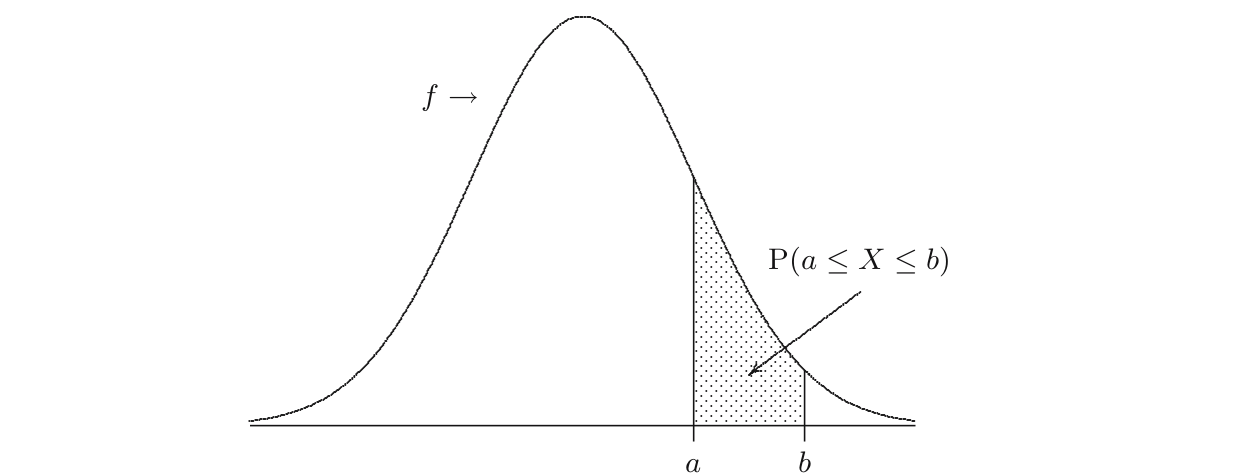
\includegraphics[width=5in,height=\textheight]{img/sc_1.png}
  \caption{ }
\end{figure} 


\begin{definition}
  Definimos al \textbf{función de distribución acumulada}, del mismo modo que
hicimos con variables discretas, pero usando ahora la integral:

\[F(x)=P(X\leq x)=\int _{-\infty }^{x}f(t)\,dt\]

\end{definition}

\subsection{Esperanza y varianza de variables continuas} 

\begin{definition}
  Para una variable aleatoria continua X con función de densidad
\(\displaystyle f(x)\) \textbf{el valor esperado o esperanza matemática}
se define como la integral

\[\displaystyle \operatorname {E} [X]=\int^{\infty}_{-\infty }xf(x)dx\]

Si recordamos es la misma idea que con variable discreta, pero en vez de
sumar integramos
\end{definition}

Al igual que ocurría con variables aleatorias discretas, en el caso continuo se cumple 

\begin{property}
  Si $X$ es una variable aleatoria continua con esperanza finita entonces se cumple que 
  \[E[a + b \cdot X] = a + b \cdot E(X)\] para cualesquiera números reales $a,b$.
\end{property}


\begin{definition}
  La \textbf{varianza} es una medida de dispersión de una variable aleatoria X respecto a su esperanza $E[X]$ y se define como la esperanza de la transformación $(X - E[X])^2$ es decir:
  
  \[Var[X]= E[(X- E[X])^2] = \int^{\infty}_{-\infty }(x-E[X])^2f(x)dx\]
\end{definition}


\begin{property}
  Si $X$ es una variable aleatoria continua con esperanza finita entonces se cumple que 
   \[
    \operatorname {Var} (X) =\operatorname {E} \left[X^{2}\right]-\operatorname {E} [X]^{2} 
 \]
\end{property}

\subsection{La distribución
uniforme} 

\begin{definition}
  
Una variable aleatoria continua tiene una distribución uniforme en el
intervalo \([\alpha, \beta]\) si función de densidad es la siguiente

\[f(x)=\begin{cases}{\frac {1}{\beta-\alpha}}&\mathrm {para} \ \alpha\leq x\leq \beta,\\[8pt]0&\text {para el resto de valores}\end{cases}\]

Se denota por \(U(\alpha, \beta)\).
\end{definition}



Si calculamos la distribución acumulada:

\[F(x)= \int _{-\infty }^{x}f(t)\,dt\]

veremos que el resultado es

\[\displaystyle F(x)=\begin{cases}0&{\text{para }}x<a\\[8pt]{\frac {x-a}{b-a}}&{\text{para }}a\leq x\leq b\\[8pt]1&{\text{para }}x>b\end{cases}\]
 

\begin{figure}[htbp]
  \begin{minipage}{0.5\linewidth}
  \centering
  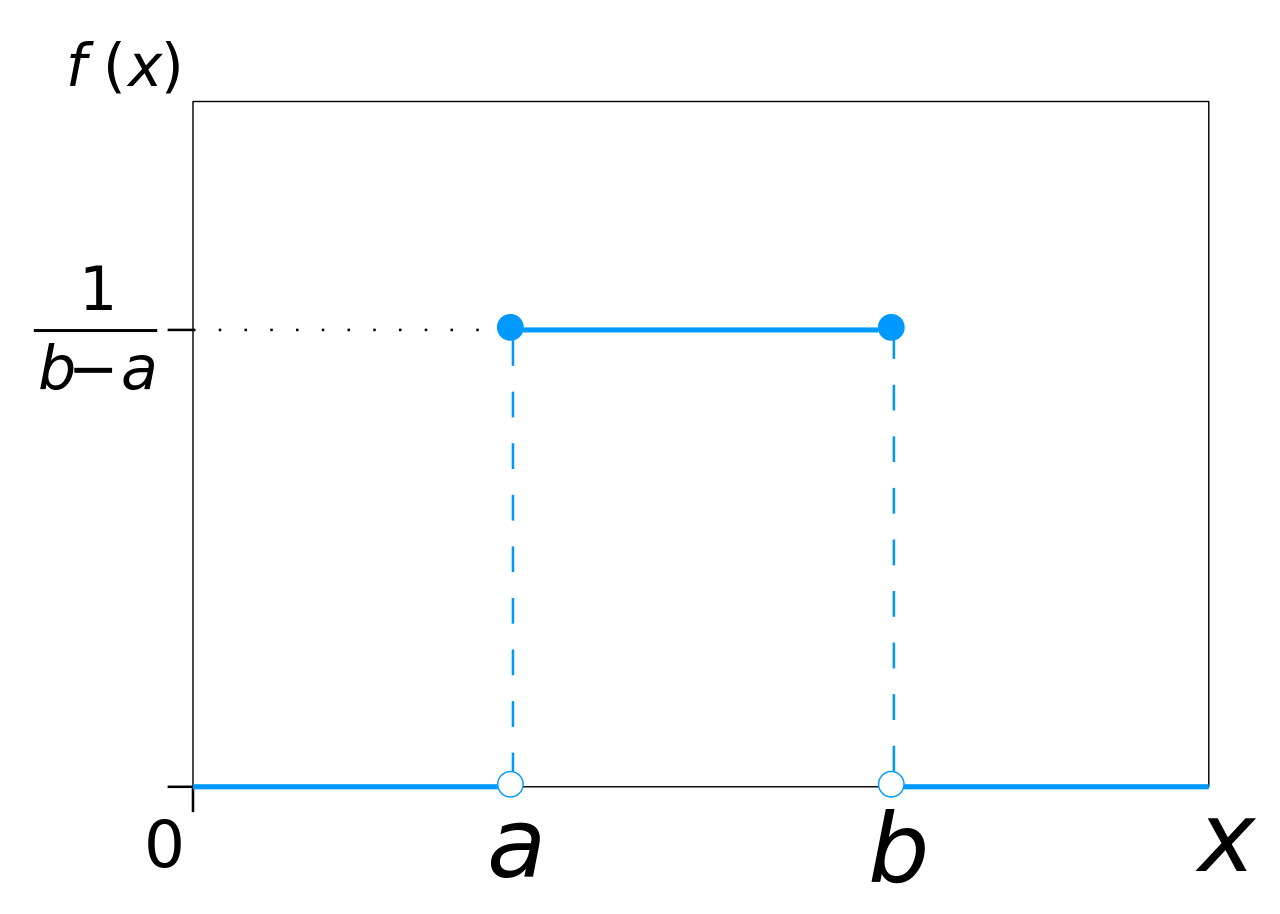
\includegraphics[width=2in,height=\textheight]{img/uniform.png}
  \caption{Función de densidad de la distribución\\ unifome}
  \end{minipage}%
  \begin{minipage}{0.5\linewidth}
  \centering
  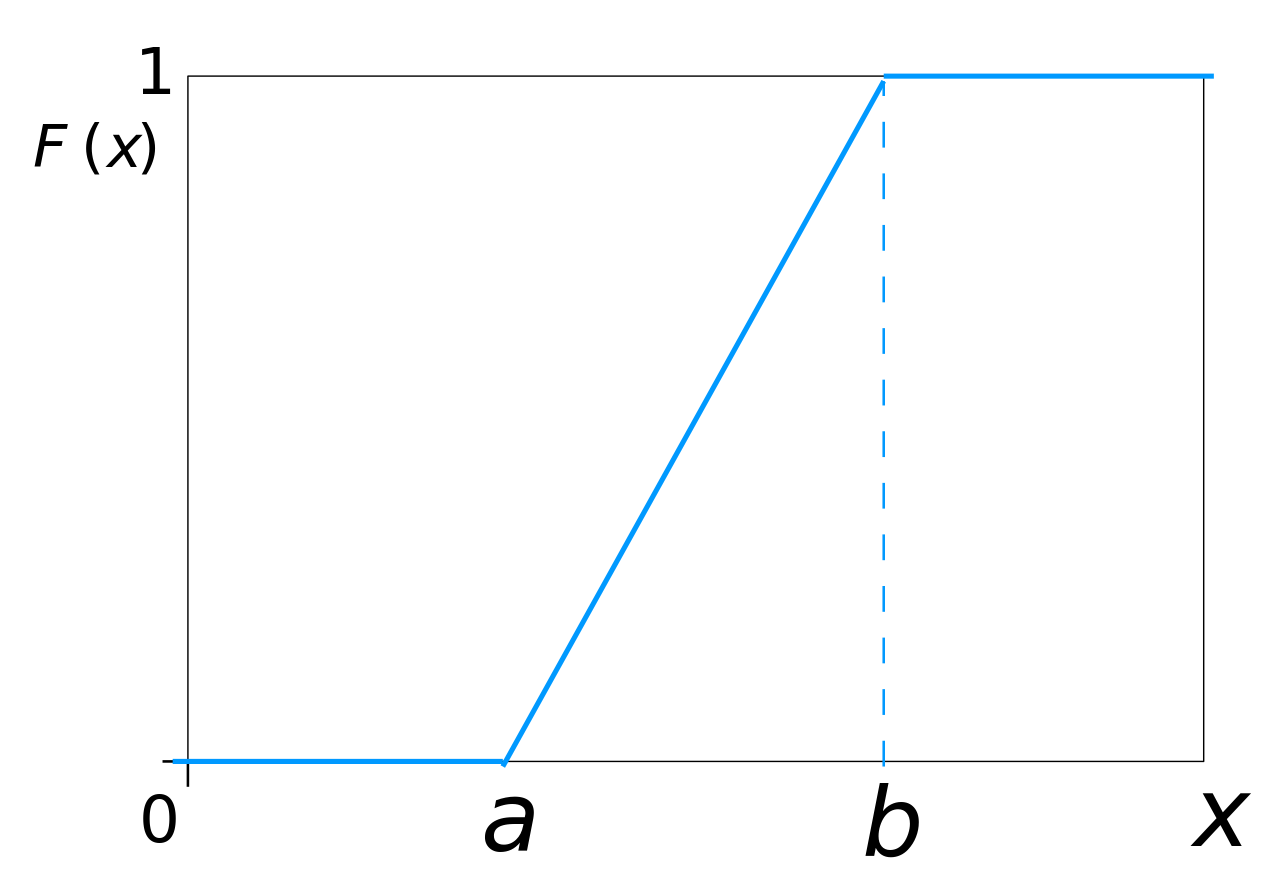
\includegraphics[width=2in,height=\textheight]{img/uniform2.png}
  \caption{Función de densidad acumulada de \\la distribución unifome}
  \end{minipage}

\end{figure} 

\begin{example}
  Para una variable  $\displaystyle X\sim U(0,23)$


  Calculemos $\displaystyle  P(2<X<18)$:

   \[\displaystyle P(2<X<18)=\int^{18}_2 \frac {1}{23-0} dx 
   =  \frac {x}{23-0} \bigg]^{18}_2 =  (18-2)\cdot {\frac {1}{23}}={\frac {16}{23}} \]
\end{example}

\begin{example}
La ruleta de la suerte tiene 20 premios repartidos en sectores iguales entre los 360 grados del círculo. Al empujar el 
la ruleta gira y finaliza al azar en cualquiera de los ángulos de giro. 
Que acabe en un ángulo concreto sigue una distribución uniforme U(0, 360). 
Calcular la probabilidad de que caiga el premio situado entre los ángulos 0 y 18 grados.
 

\[\displaystyle P(0<X<18)=\int^{18}_0 \frac {1}{360-0} dx 
=  \frac {x}{360} \bigg]^{18}_0 =  (18-0)\cdot {\frac {1}{360}}={\frac {18}{360}} \]

\end{example}

\begin{property}
  Si $X \sim  U(\alpha, \beta)$ entonces 
  \begin{enumerate}
    \item $E[X] = \frac{1}{2} (\alpha+\beta)$
    \item $V[X] = \frac{1}{12} (\beta-\alpha)$
  \end{enumerate}
\end{property}

\begin{proof}
  Para ver (1), basta calcular 
  \[E[X] = \int^{\beta}_{\alpha} x \frac{1}{\beta - \alpha} dx 
  = \bigg[\frac{x^2}{2}\bigg]^{\beta}_{\alpha}\frac{1}{\beta - \alpha}  =  \frac{\beta^2-\alpha^2}{2(\beta - \alpha)}
  = \frac{(\beta-\alpha)(\beta + \alpha)}{2(\beta - \alpha)} = \frac{1}{2} (\alpha+\beta) \]
  Para demostrar (2) usaremos que $E[X^2] = \frac{\beta^3 - \alpha^3}{3\beta - 3\alpha}$, esto se puede demostrar usando una integral similar a la anterior. 
  Ahora vemos que 
  \begin{align*}
    V[X] &= E[X^2] - E[X]^2 = \frac{\beta^3 - \alpha^3}{3\beta-3\alpha} - \frac{(\alpha+\beta)^2}{4} \\
    &= \frac{4(\beta^3 - \alpha^3) - 3(\beta-\alpha)(\alpha+\beta)^2}{12(\beta-\alpha)} \\
    &= \frac{(\beta-\alpha)^3}{12(\beta - \alpha)} = \frac{1}{12} (\beta-\alpha)
  \end{align*}
 
\end{proof}


\subsection{La distribución exponencial} 

\begin{definition}
  Una variable aleatoria continua tiene una distribución \textbf{exponencial} de parámetro 
  $\lambda$ si su función de densidad es la siguiente
  
  \[f(x)=\begin{cases}
    \lambda e^{-\lambda x} &\mathrm {para} \ x\geq 0,\\
     0&\text {para el resto de valores}
  \end{cases}\]
  
  Se denota por \(exp(\lambda)\).
\end{definition}

\begin{figure}[htbp]
  \begin{minipage}{0.5\linewidth}
  \centering
  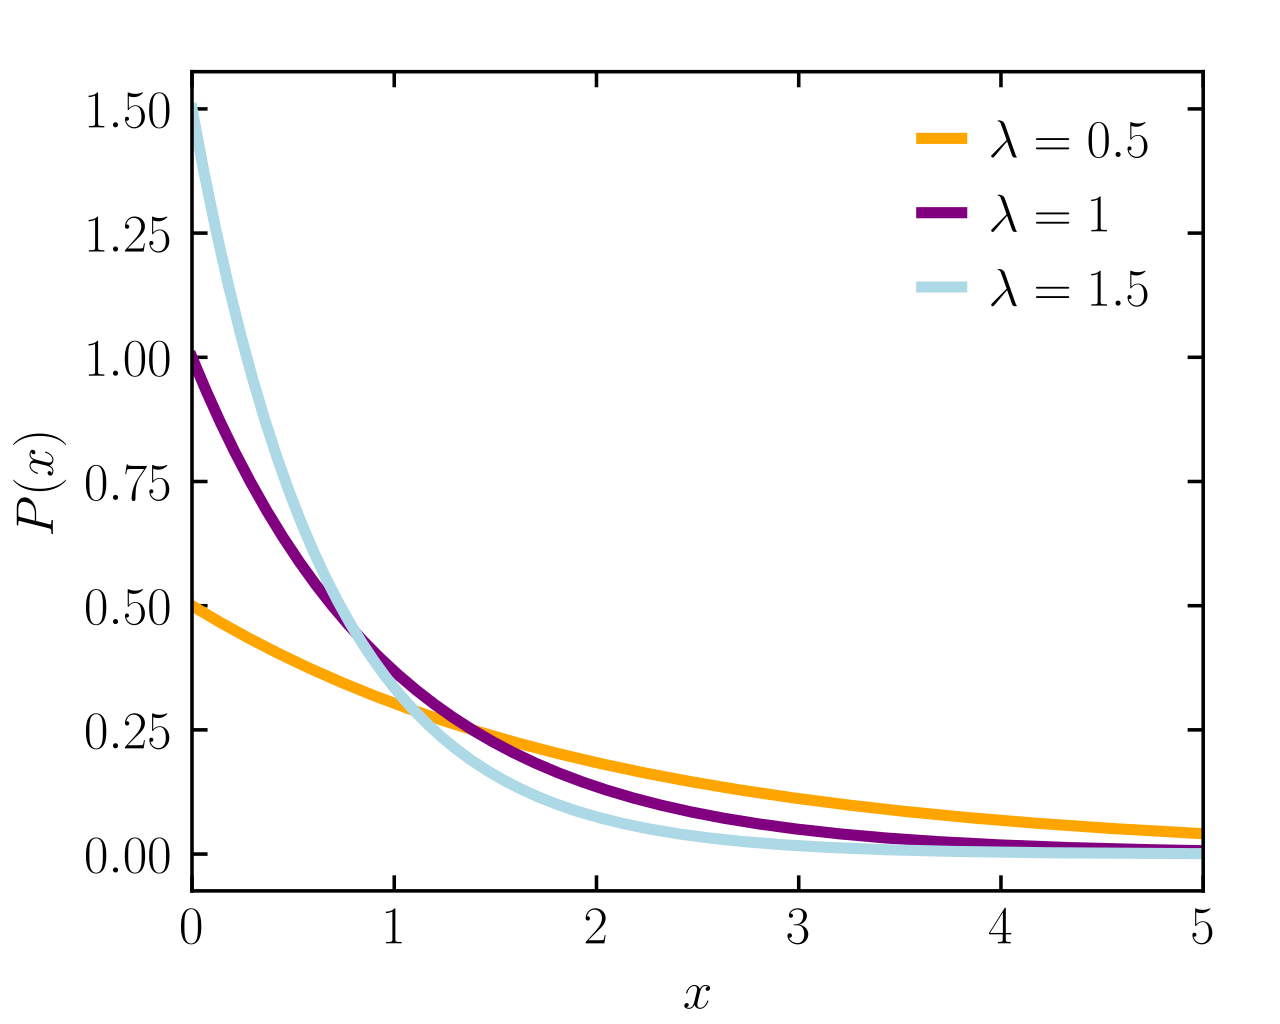
\includegraphics[width=2in,height=\textheight]{img/exponential_distribution1.png}
  \caption{Función de densidad de la distribución\\ exponencial}
  \end{minipage}%
  \begin{minipage}{0.5\linewidth}
  \centering
  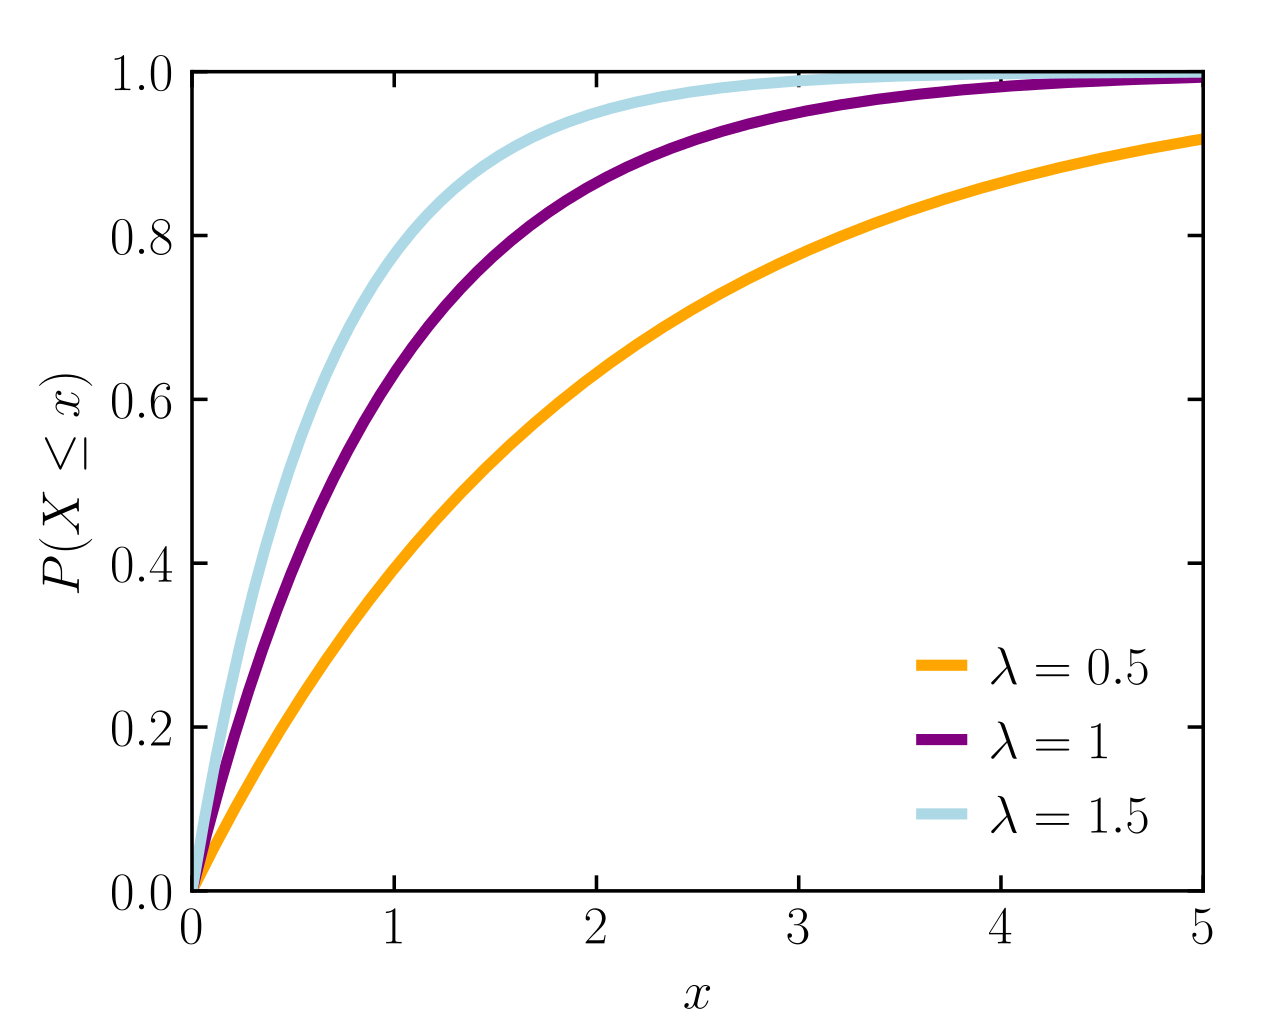
\includegraphics[width=2in,height=\textheight]{img/exponential_distribution2.png}
  \caption{Función de densidad acumulada de \\la distribución exponencial}
  \end{minipage}

\end{figure} 


\begin{property}\label{prop_exp_mean}
  Si $X \sim  exp(\lambda)$ entonces 
  \begin{enumerate}
    \item $E[X] = \frac{1}{\lambda}$
    \item $V[X] = \frac{1}{\lambda^2}$
  \end{enumerate}
\end{property}

\begin{proof}
  \[E[X] = \int^{\infty}_{0} \lambda x e^{-\lambda x} dx 
  = \lim_{y\to \infty}\lambda \bigg[ e^{-\lambda x} \frac{x \lambda -1}{\lambda^2}\bigg]^y_0 = \lim_{y\to \infty} \big( e^{-\lambda y }\frac{y\lambda -1}{\lambda} + \frac{1}{\lambda}\big) = \frac{1}{\lambda} \]

  Para resolver esta integral hemos usado que $\int x e^{cx} dx = e^{c x } \frac{c x - 1}{c ^2} + c$

  Para calcular la varianza aplicando integración por partes con $u = \lambda x^2$ y $v = e^{\lambda x }$, podemos ver facilmente que 

  \[E[X^2] = \int^{\infty}_{0} \lambda x^2 e^{-\lambda x} dx = 2/\lambda^2\]

  (omitimos los detalles de la anterior integral), y de este modo
  
  \[V[X] = E[X^2] - E[X]^2 = \frac{2}{\lambda^2} - \frac{1}{\lambda^2} = \frac{1}{\lambda^2}\]
\end{proof}


\begin{example}
  El número de kilómetros viajados por un coche hasta que la transmisión se rompe sigue una variable
  $exp(\lambda= 1/100 000)$. 
  \begin{enumerate}[(1)]
    \item ¿Cuál es la probabilidad de que se roma antes de los $50000$ kilómetros?
    \item ¿Cuál es el número esperado de kilómetros hasta que se rompa?
  \end{enumerate}

  Para resolver (1) pensemos en que 
  \begin{align*}
    P(X\leq 50000) &= \int^{50000}_0 \frac{1}{100000} e ^{\frac{-1}{100000}x} dx\\
    &=\big[ - e^{\frac{-x}{100000}}\big]^{50000}_0  = 1 - e^{-1/2} \cong 0.393
  \end{align*}

  Para (2) aplicamos la propiedad anterior \ref{prop_exp_mean}(1), con lo que 
  \[E[X] = 1/\lambda = 100000\] 
 
\end{example}

\begin{customdef}{Aplicaciones de la distribución exponencial}
  La distribución exponencial puede ser interpretada como la versión continua de la distribución geométrica. A diferencia de la 
  distribución geométrica (que recordemos era el número de intentos hasta el primer acierto en un experimento de Bernoulli), 
  la exponencial describe \emph{el tiempo necesario para que un proceso continuo cambie su estado}

  Para eventos que ocurren a un ritmo constante, con una "media de tiempo necesario para que ocurra" conocida, a distribución exponencial 
  puede usarse para estudiar el \emph{tiempo hasta la siguiente ocurrencia de ese evento}. 

  Algunos ejemplos de usos de la exponencial pueden ser 
  \begin{itemize}
    \item tiempo necesario hasta que llegue el próximo consumidor a una tienda
    \item tiempo hasta siguiente fallo del sistema
    \item tiempo hasta que aparezca el siguiente rayo en una tormenta
    \item kilómetros hasta que se estropee una pieza de un motor.
    \item $\ldots$
  \end{itemize}
\end{customdef}

\subsection{La distribución normal} 

La distribución normal juega un rol central en la teoría de la
probabilidad y la estadística. Una de sus aplicaciones se debe a C.F.
Gauss, que la usó en 1809 para medir errores en astronomía.

\begin{definition}
  
Una función aleatoria continua tiene una \textbf{distribución normal}
con parámetros \(\mu\) y \(\sigma\), su función de densidad de
probabilidad es

\begin{equation}\label{eq_nmusigma}
  f(x) = \frac{1}{\sigma \sqrt{2\pi}} e^{-\frac{(x-\mu)^2}{2\sigma^2}}
\end{equation}
 

Esta distribución se denota por \(N(\mu, \sigma^2)\).
\end{definition}

\begin{figure}[htbp]
  \begin{minipage}{0.5\linewidth}
  \centering
  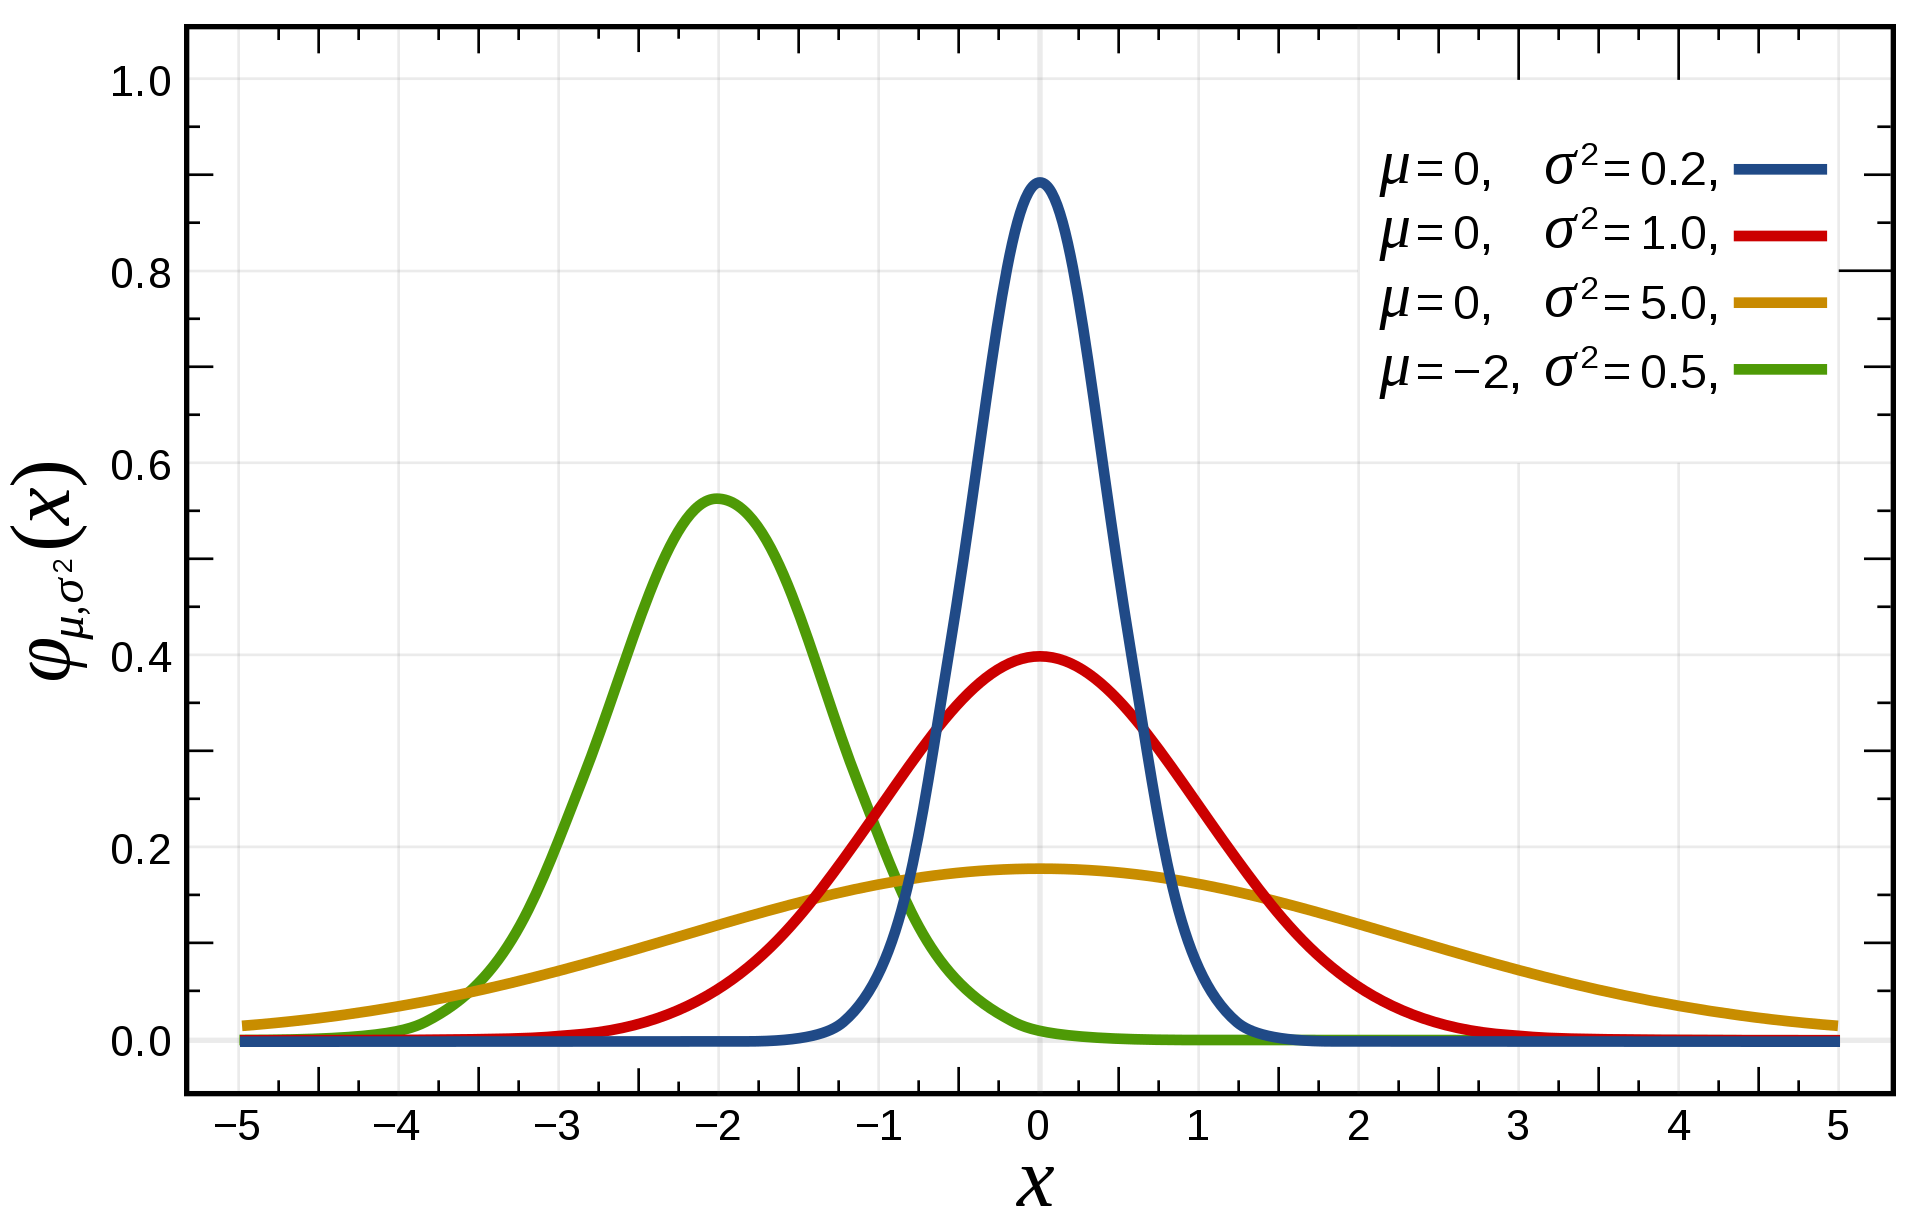
\includegraphics[width=2in,height=\textheight]{img/normal1_new.png}
  \caption{Función de densidad de la distribución\\ normal}
  \end{minipage}%
  \begin{minipage}{0.5\linewidth}
  \centering
  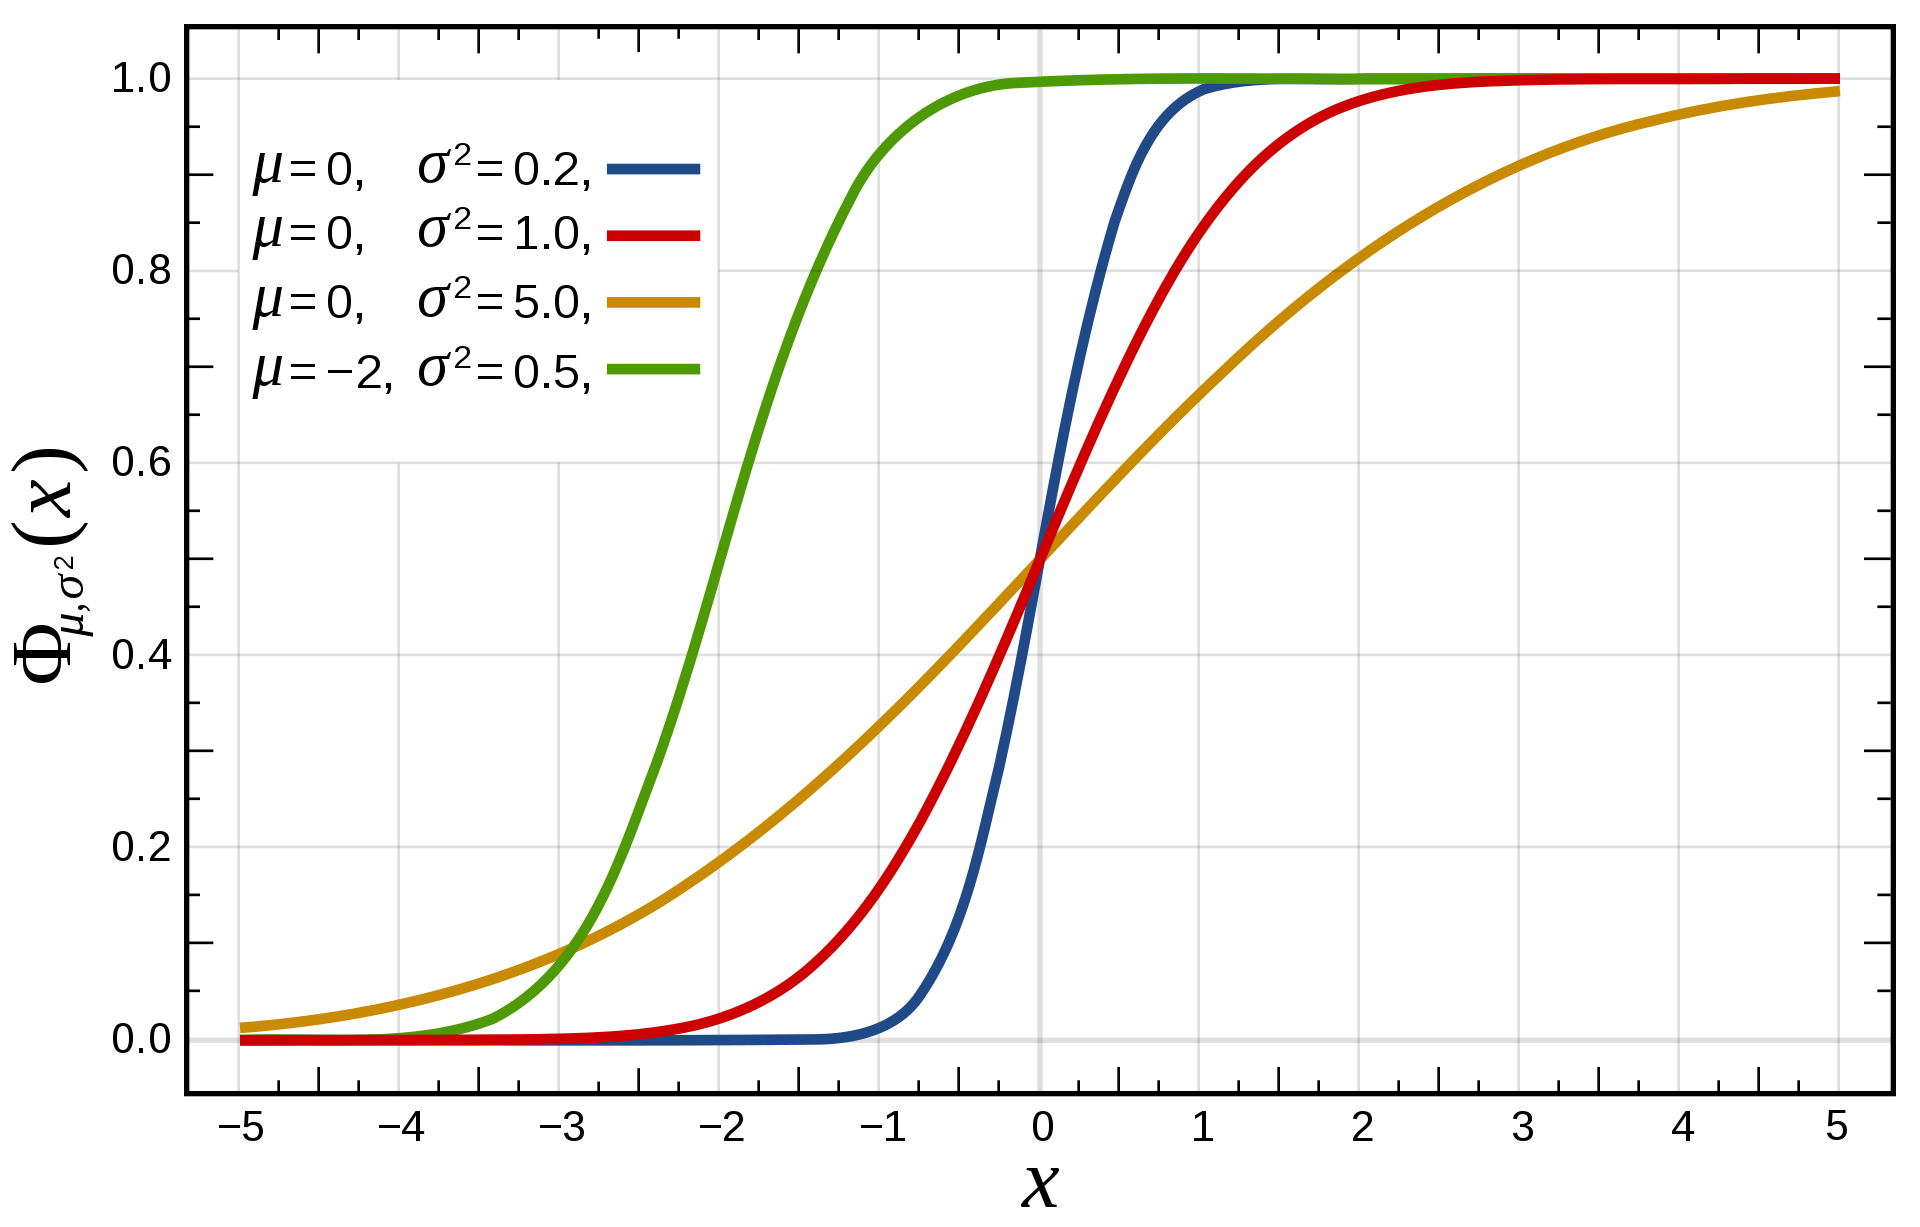
\includegraphics[width=2in,height=\textheight]{img/normal2_new.png}
  \caption{Función de densidad acumulada de \\la distribución normal}
  \end{minipage}
\end{figure} 


\begin{customdef}{Interpretación de $\mu$ y $\sigma$}

Como vemos esta función \(f\) tiene una forma de campana, donde los
parámetros \(\mu\) y \(\sigma\) se interpretan como:

\begin{itemize}
\item
  \(\mu\) determina el valor entorno al que se centra la campana.
  Veremos que coincide con la esperanza matemática. Este valor es el valor en torno al cual se sitúa la campana, su máximo.
\item
  \(\sigma\) determina lo \emph{apretada o esparcida} que está la campana, es decir
  lo dispersa que está la variable. Valores más grandes de $\sigma$ darán lugar a campanas más abiertas.
\end{itemize}

\end{customdef}


\begin{customdef}{Aplicaciones de la Normal}
Algunos ejemplos de variables asociadas a fenómenos naturales que siguen
el modelo de la normal son:

\begin{itemize}
\item
  caracteres morfológicos de individuos como la estatura;
\item
  caracteres fisiológicos como el efecto de un fármaco;
\item
  caracteres sociológicos como el consumo de cierto producto por un
  mismo grupo de individuos;
\item
  caracteres psicológicos como el cociente intelectual;
\item
  nivel de ruido en telecomunicaciones;
\item
  errores cometidos al medir ciertas magnitudes;
  \item $\cdots$
\end{itemize}
\end{customdef}

\begin{property}
  Si $X \sim  N(\mu, \sigma^2)$ entonces 
  \begin{enumerate}
    \item $E[X] = \mu$
    \item $V[X] = \sigma^2$
  \end{enumerate}
\end{property}

\begin{proof}
   
\end{proof}

\subsubsection*{La normal N(0,1)}

La versión de la normal más sencilla de todas es la que tiene $\mu=0$ y $\sigma = \sigma^2 = 1$.

\begin{equation}\label{eq_n01}
  f(z) = \frac{1}{\sqrt{2\pi}} e^{-\frac{z}{2}}
\end{equation}
  
Como veremos a menudo podemos usar esta normal para trabajar con cualquier otra normal con parámetros cualesquiera $\mu, \sigma$.



Usando \ref{eq_n01}, definimos:

\begin{equation}\label{eq_phi_norm}
  \Phi(y) = \int^{\infty}_{y} f(z)dz
\end{equation}
 

Que coincidirá con el área bajo
la curva:
 
\begin{figure}[htbp]
  \centering
  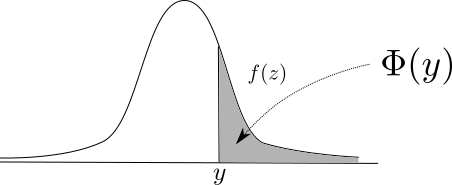
\includegraphics[width=2in,height=\textheight]{img/drawing_phi.png}
  \caption{$\Phi$}
\end{figure} 


\begin{customdef}{Uso de la Normal $N(0,1)$ para calcular probabilidades de normales $N(\mu, \sigma)$}

Supongamos que tenemos una variable aleatoria $X \sim N(\mu, \sigma)$. Podemos considerar la nueva variable

\[Z = \frac{X-\mu}{\sigma}\]

Veamos cómo calcular la probabilidad de que $X$ tome valores en un intervalo $(a, b)$ usando la normal $N(0,1)$.

Considerando  
\begin{align*}
  z_a &=(a-\mu)/\sigma\\
  z_b&=(b-\mu)/\sigma
\end{align*}

 vemos que 

\begin{align*}
    P(a\leq X\leq b)&= \int^b_a f(x) dx \\
    &= \int^b_a \frac{1}{\sigma \sqrt{2\pi}} e^{-\frac{(x-\mu)^2}{2\sigma^2}} dx
    = \int^{b}_{a} \frac{1}{\sigma \sqrt{2\pi}} e^{-\frac{1}{2}\big(\frac{x-\mu}{\sigma}\big)^2} dx
    = \int^{z_b}_{z_a} \frac{1}{\sigma \sqrt{2\pi}} e^{-\frac{z^2}{2}} dz\\ 
    &= \int^{z_b}_{z_a} f(z) dz = \bigg(\int^{\infty}_{z_a} f(z) dz\bigg) - \bigg(\int^{\infty}_{z_b} f(z) dz\bigg)  = \Phi(z_a) - \Phi(z_b)
\end{align*}

Hemos las propiedades de la integral definida sobre la ecuación \ref{eq_nmusigma}, haciendo el cambio de
variable $z=(x-\mu)/\sigma$ y c.
\end{customdef}

\begin{example}
  La distribución de estaturas de un conjunto de personas se ajusta a un
modelo normal \(N(169cm,8cm)\). Se pide:
\begin{enumerate}
  \item la probabilidad de que una persona tenga su estatura comprendida entre 171 y 175 cm
\end{enumerate}

En este caso tenemos que \(b = 175, a =171\) y
\(z_b = (175-169)/8=0.75, z_a = (171-169)/8=0.25\) De acuerdo con
lo anterior, basta
con calcular
\(P(a\leq X\leq b) = (\Phi(z_a) - \Phi(z_b))= \Phi(0.25) - \Phi(0.75)\)
para obtener el resultado, buscando los valores en la tabla obtenemos que el s
\(\Phi(0.25) - \Phi(0.75) =   (0.40129 - 0.22965)\) 

\end{example}


\newpage


\textbf{Tabla de valores Normal \(N(0,1)\)}\\
el valor de la tabla es \(\Phi(y) = \int^{\infty}_{y} f(z)dz\). Sobre el
lado de las filas los primeros dos decimales, sobre las columnas los
siguientes.

Si queremos buscar el valor \(\Phi(0.12)\) debemos fijarnos en el valor
que está sobre la fila 2 (que comienza con \(0.1\)) y la columna 3 (que
comienza con \(+0.02\)), lo que nos da \(0.45224\)

Para valores negativos tener en cuenta que \(\Phi(-y) = 1-\Phi(y)\).
Luego si por ejemplo queremos calcular \(\Phi(-0.12)\) basta con buscar
\(\Phi(0.12)\) y luego calcular \(1-\Phi(0.12)\)\\



\begin{longtable}[]{@{}ccccccccccc@{}}
\toprule
y & +0.00 & +0.01 & +0.02 & +0.03 & +0.04 & +0.05 & +0.06 & +0.07 &
+0.08 & +0.09\tabularnewline
\midrule
\endhead
0.0 & 0.50000 & 0.49601 & 0.49202 & 0.48803 & 0.48405 & 0.48006 &
0.47608 & 0.47210 & 0.46812 & 0.46414\tabularnewline
0.1 & 0.46017 & 0.45620 & 0.45224 & 0.44828 & 0.44433 & 0.44038 &
0.43640 & 0.43251 & 0.42858 & 0.42465\tabularnewline
0.2 & 0.42074 & 0.41683 & 0.41294 & 0.40905 & 0.40517 & 0.40129 &
0.39743 & 0.39358 & 0.38974 & 0.38591\tabularnewline
0.3 & 0.38209 & 0.37828 & 0.37448 & 0.37070 & 0.36693 & 0.36317 &
0.35942 & 0.35569 & 0.35197 & 0.34827\tabularnewline
0.4 & 0.34458 & 0.34090 & 0.33724 & 0.33360 & 0.32997 & 0.32636 &
0.32276 & 0.31918 & 0.31561 & 0.31207\tabularnewline
0.5 & 0.30854 & 0.30503 & 0.30153 & 0.29806 & 0.29460 & 0.29116 &
0.28774 & 0.28434 & 0.28096 & 0.27760\tabularnewline
0.6 & 0.27425 & 0.27093 & 0.26763 & 0.26435 & 0.26109 & 0.25785 &
0.25463 & 0.25143 & 0.24825 & 0.24510\tabularnewline
0.7 & 0.24196 & 0.23885 & 0.23576 & 0.23270 & 0.22965 & 0.22663 &
0.22363 & 0.22065 & 0.21770 & 0.21476\tabularnewline
0.8 & 0.21186 & 0.20897 & 0.20611 & 0.20327 & 0.20045 & 0.19766 &
0.19489 & 0.19215 & 0.18943 & 0.18673\tabularnewline
0.9 & 0.18406 & 0.18141 & 0.17879 & 0.17619 & 0.17361 & 0.17106 &
0.16853 & 0.16602 & 0.16354 & 0.16109\tabularnewline
1.0 & 0.15866 & 0.15625 & 0.15386 & 0.15151 & 0.14917 & 0.14686 &
0.14457 & 0.14231 & 0.14007 & 0.13786\tabularnewline
1.1 & 0.13567 & 0.13350 & 0.13136 & 0.12924 & 0.12714 & 0.12507 &
0.12302 & 0.12100 & 0.11900 & 0.11702\tabularnewline
1.2 & 0.11507 & 0.11314 & 0.11123 & 0.10935 & 0.10749 & 0.10565 &
0.10383 & 0.10204 & 0.10027 & 0.09853\tabularnewline
1.3 & 0.09680 & 0.09510 & 0.09342 & 0.09176 & 0.09012 & 0.08851 &
0.08692 & 0.08534 & 0.08379 & 0.08226\tabularnewline
1.4 & 0.08076 & 0.07927 & 0.07780 & 0.07636 & 0.07493 & 0.07353 &
0.07215 & 0.07078 & 0.06944 & 0.06811\tabularnewline
1.5 & 0.06681 & 0.06552 & 0.06426 & 0.06301 & 0.06178 & 0.06057 &
0.05938 & 0.05821 & 0.05705 & 0.05592\tabularnewline
1.6 & 0.05480 & 0.05370 & 0.05262 & 0.05155 & 0.05050 & 0.04947 &
0.04846 & 0.04746 & 0.04648 & 0.04551\tabularnewline
1.7 & 0.04457 & 0.04363 & 0.04272 & 0.04182 & 0.04093 & 0.04006 &
0.03920 & 0.03836 & 0.03754 & 0.03673\tabularnewline
1.8 & 0.03593 & 0.03515 & 0.03438 & 0.03362 & 0.03288 & 0.03216 &
0.03144 & 0.03074 & 0.03005 & 0.02938\tabularnewline
1.9 & 0.02872 & 0.02807 & 0.02743 & 0.02680 & 0.02619 & 0.02559 &
0.02500 & 0.02442 & 0.02385 & 0.02330\tabularnewline
2.0 & 0.02275 & 0.02222 & 0.02169 & 0.02118 & 0.02068 & 0.02018 &
0.01970 & 0.01923 & 0.01876 & 0.01831\tabularnewline
2.1 & 0.01786 & 0.01743 & 0.01700 & 0.01659 & 0.01618 & 0.01578 &
0.01539 & 0.01500 & 0.01463 & 0.01426\tabularnewline
2.2 & 0.01390 & 0.01355 & 0.01321 & 0.01287 & 0.01255 & 0.01222 &
0.01191 & 0.01160 & 0.01130 & 0.01101\tabularnewline
2.3 & 0.01072 & 0.01044 & 0.01017 & 0.00990 & 0.00964 & 0.00939 &
0.00914 & 0.00889 & 0.00866 & 0.00842\tabularnewline
2.4 & 0.00820 & 0.00798 & 0.00776 & 0.00755 & 0.00734 & 0.00714 &
0.00695 & 0.00676 & 0.00657 & 0.00639\tabularnewline
2.5 & 0.00621 & 0.00604 & 0.00587 & 0.00570 & 0.00554 & 0.00539 &
0.00523 & 0.00508 & 0.00494 & 0.00480\tabularnewline
2.6 & 0.00466 & 0.00453 & 0.00440 & 0.00427 & 0.00415 & 0.00402 &
0.00391 & 0.00379 & 0.00368 & 0.00357\tabularnewline
2.7 & 0.00347 & 0.00336 & 0.00326 & 0.00317 & 0.00307 & 0.00298 &
0.00289 & 0.00280 & 0.00272 & 0.00264\tabularnewline
2.8 & 0.00256 & 0.00248 & 0.00240 & 0.00233 & 0.00226 & 0.00219 &
0.00212 & 0.00205 & 0.00199 & 0.00193\tabularnewline
2.9 & 0.00187 & 0.00181 & 0.00175 & 0.00169 & 0.00164 & 0.00159 &
0.00154 & 0.00149 & 0.00144 & 0.00139\tabularnewline
3.0 & 0.00135 & 0.00131 & 0.00126 & 0.00122 & 0.00118 & 0.00114 &
0.00111 & 0.00107 & 0.00104 & 0.00100\tabularnewline
3.1 & 0.00097 & 0.00094 & 0.00090 & 0.00087 & 0.00084 & 0.00082 &
0.00079 & 0.00076 & 0.00074 & 0.00071\tabularnewline
3.2 & 0.00069 & 0.00066 & 0.00064 & 0.00062 & 0.00060 & 0.00058 &
0.00056 & 0.00054 & 0.00052 & 0.00050\tabularnewline
3.3 & 0.00048 & 0.00047 & 0.00045 & 0.00043 & 0.00042 & 0.00040 &
0.00039 & 0.00038 & 0.00036 & 0.00035\tabularnewline
3.4 & 0.00034 & 0.00032 & 0.00031 & 0.00030 & 0.00029 & 0.00028 &
0.00027 & 0.00026 & 0.00025 & 0.00024\tabularnewline
3.5 & 0.00023 & 0.00022 & 0.00022 & 0.00021 & 0.00020 & 0.00019 &
0.00019 & 0.00018 & 0.00017 & 0.00017\tabularnewline
3.6 & 0.00016 & 0.00015 & 0.00015 & 0.00014 & 0.00014 & 0.00013 &
0.00013 & 0.00012 & 0.00012 & 0.00011\tabularnewline
3.7 & 0.00011 & 0.00010 & 0.00010 & 0.00010 & 0.00009 & 0.00009 &
0.00008 & 0.00008 & 0.00008 & 0.00008\tabularnewline
3.8 & 0.00007 & 0.00007 & 0.00007 & 0.00006 & 0.00006 & 0.00006 &
0.00006 & 0.00005 & 0.00005 & 0.00005\tabularnewline
3.9 & 0.00005 & 0.00005 & 0.00004 & 0.00004 & 0.00004 & 0.00004 &
0.00004 & 0.00004 & 0.00003 & 0.00003\tabularnewline
4.0 & 0.00003 & 0.00003 & 0.00003 & 0.00003 & 0.00003 & 0.00003 &
0.00002 & 0.00002 & 0.00002 & 0.00002\tabularnewline
\bottomrule
\end{longtable}

\end{document}